\documentclass{article}
\usepackage[utf8]{inputenc}
\usepackage[brazilian]{babel}
\usepackage{subfigure}

\title{Sistema de arquivos}
\author{João Vitor, Millas Násser, Welton Santos}
\date{Dezembro 2017}

\usepackage{natbib}
\usepackage{graphicx}

\begin{document}

\maketitle

\section{Introdução}
	O trabalho apresenta uma simulação de um sistema de arquivo simples que é baseado em uma tabela de entradas. Utilizando de estruturas especiais que simulam a memória principal e um arquivo simulando o disco, além de tipos de dados que implementam diretórios e arquivos, cada entrada da tabela possui 16 bits e  armazena o endereço dos blocos de arquivos. 
	
	O objetivo principal é realizar a simulação e verificar a granularidade do disco ao final de uma série de comandos, a fim de verificar a fragmentação gerada.
	
\section{A FAT-16}
	O sistema de arquivos FAT-16 consiste em uma tabela que armazena quais os endereços de um arquivo. Uma posição na FAT armazena qual é o próximo bloco a ser acessado para realizar a leitura de um arquivo.
	
	\begin{figure}[!h]
		\centering
		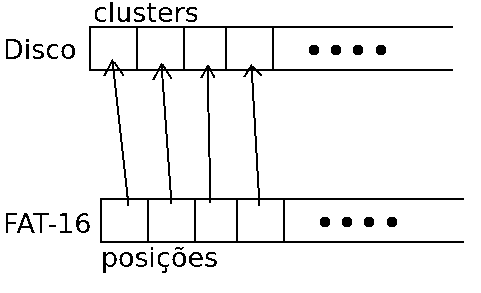
\includegraphics[scale=0.5]{mapeamentoFatDisco.png}
		\caption{Mapeamento de endereços da FAT-16 para \textit{clusters} do disco}
		\label{fig:fatDisc}
	\end{figure}

	A ideia principal é mapear todas as entradas do disco para uma tabela que o armazena. Para isso cada entrada do sistema de arquivos mapeia um \textit{cluster} do disco (1024 bytes) e no total o disco possui 4096 entradas e 10 destas são utilizadas para o mapeamento de uma região conhecida do disco para que ele possa dar boot no sistema operacional. Nesta região possui 3 áreas especiais:
	\begin{itemize}
	 \item \textit{Boot block}
	 \item \textit{FAT-16}
	 \item \textit{Diretório Root}
	\end{itemize}
	Onde o \textit{Boot block} possui a função de indicar o início dos \textit{clusters} conhecidos para o \textit{boot}, utiliza-se 1 \textit{cluster}. Os próximos 9 \textit{clusters} são para a persistir a FAT no disco, e por fim 1 \textit{cluster} para o diretório root.
	
	Visto que existem 4086 \textit{clusters} disponíveis para escrita livre, a Figura \ref{fig:fatDisc} representa sucintamente o mapeamento da FAT para as posições livres dentro do disco onde cada posição da FAT há um \textit{cluster} correspondente, levando a um mapeamento direto.
	
	Há dois tipos de arquivos que podem ser escritos na FAT-16, diretórios e arquivos de dados. O primeiro consome sempre um \textit{cluster} do disco, já arquivos podem consumir mais que um \textit{cluster}. Para o sistema de arquivos resolver estes arquivos se utiliza do mapeamento direto e utilizar as posições da FAT como ponteiros para próximas posições do arquivo, tal como representado na figura \ref{fig:arqDirDisc}.
	
	\begin{figure}[!h]
		\centering
		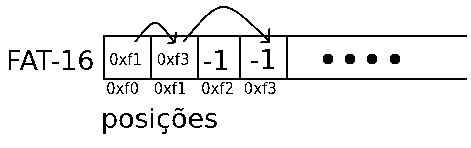
\includegraphics[scale=0.5]{mapeamentoArqDir.png}
		\caption{Mapeamento de um arquivo pela FAT-16 com as respectivas posições utilizadas}
		\label{fig:arqDirDisc}
	\end{figure}

	Segundo a imagem um arquivo qualquer que inicia no cluster \textit{0xf0}, ao acessar a posição correspondente na FAT o conteúdo é o endereço da próxima posição que deve ser acessada para continuar a ler o arquivo, que é o endereço \textit{0xf1}, e assim por diante até encontrar o valor -1 que representa o final de um arquivo, a cada leitura de uma posição da FAT-16 é lido também o respectivo \textit{cluster} no disco com o conteúdo do arquivo. Arquivos que na primeira posição da FAT-16 já possuem -1 indicam que seu tamanho é de apenas 1 \textit{cluster}, tal como em 0xf2.
	
	
	
\section{Simulador FAT-16} 
	A proposta deste simulador é providenciar recursos suficientes para analisar o desempenho do sistema de arquivos FAT-16, em relação a pesquisa e alocação de memória secundária. A memória secundária será por completa simulada através de um arquivo de texto fornecendo acesso aleatório. 

\section{Sistema de Arquivos} 
	Sistema de arquivos é uma camada de software entre o hardware e o sistema operacional, responsável por criar uma abstração de hierarquia de arquivos para facilitar a manipulação pelo sistema operacional e também pelos usuários. O sistema de arquivos defini como uma partição organiza seus arquivos, quais recursos estão disponíveis, limite no tamanho de arquivos e diretórios, atributos de um arquivo, sistema de proteção contra falhas dentre outros parâmetros não relevantes ao contexto. Existem vários sistemas de arquivos para diversas situações e neste trabalho será abordado o sistema FAT-16, presente no sistema MS-DOS e Windows 95. 

\section{FAT - File Allocation Table} 
	FAT, consiste em um sistema de arquivos dentre vários outros existentes \textit{(vfat, ext, ntfs, ufs etc...)}, atualmente mais utilizado em mídias de menor capacidade como pendrives e memória para dispositivos com sistemas embarcados isso devido a algumas limitações como a baixa segurança contra perda de dados, limitação no tamanho de arquivos (limite de 2GB para FAT-16 com bloco de 32KB) e principalmente o alto consumo de memória necessário para gerenciar mídias com capacidade de armazenamento elevadas (Disco Rígidos atuais). 
	A gerência de arquivos é feita através de uma tabela situada em uma região separada na partição contendo referência para todos os blocos de dados.  

\subsection{Fragmentação (Alocação Contígua x FAT)} 
	Considerado fundamental, o acesso á aleatório a memória é um recurso que permite a um usuário alterar o estado de um arquivo persistido. Diferente da alocação contígua, um arquivo pode ter seu conteúdo expandido, removido ou até mesmo excluído da mídia de armazenamento sem que gere grande desperdício de espaço, ocorrido no método de alocação contígua onde o surgimento lacunas (trechos de memória não utilizadas) é comum. A existência de lacunas dificulta a reutilização da memória logo que é provinda geralmente pela exclusão de arquivos com tamanhos distintos, raramente encontra-se outro arquivo com o tamanho exato ao do removido para ocupar o espaço liberado, e este fator causa o problema da \textbf{segmentação externa}. 
	Apesar da melhor gestão de memória apresentada, a leitura em sistemas de alocação contígua é mais eficiente, devido a disposição linear dos dados na mídia. Esta forma de alocação evita gastos excessivos como o movimento do braço de um disco rígido para diferentes regiões em curtos intervalos de tempo, necessário para lidar com a \textbf{segmentação interna} do arquivo. Portanto pode-se dizer que a grande vantagem da FAT em economia de memória é descontada na velocidade de pesquisa em relação a alocação contígua. 

\subsection{Acesso Aleatório} 
	Outra vantagem é a facilidade na pesquisa, para acessar regiões aleatórias de um arquivo o mesmo não precisa de ser enviado por completo para memória, permitindo que trechos menores do arquivo sejam carregados conforme a necessidade, dispensando o gasto computacional para encontrar trechos específicos, o que é comum em sistemas como o presente em CD's-ROM (Read Only Memory), onde é sempre necessário uma pesquisa linear pelo CD para encontrar o dado desejado. Para dispositivos com memória reduzida esta qualidade é um diferencial crucial. 

\subsection{Disposição dos arquivos}
    
\section{Conclusão}
    
\end{document}
